\chapter{Listas enlazadas}

En esta unidad nos dedicaremos a construir nuestras propias listas, que
consistirán de cadenas de objetos enlazadas mediante referencias, como las
vistas en la unidad anterior.

Si bien Python ya cuenta con sus propias listas, las listas enlazadas que
implementaremos en esta unidad nos resultarán también útiles.

\section{Una clase sencilla de {\it vagones}}

En primer lugar, definiremos una clase muy simple, \lstinline!Nodo!, que se
comportará como un vagón: tendrá sólo dos atributos: \lstinline!dato!, que
servirá para almacenar cualquier información, y \lstinline!prox!, que servirá
para poner una referencia al siguiente vagón.

Además, como siempre, implementaremos el constructor y el método
\lstinline!__str__! para poder obtener una representación en cadena de texto.

\begin{codigo-python-sn}
class Nodo:
    def __init__(self, dato=None, prox=None):
        self.dato = dato
        self.prox = prox

    def __str__(self):
        return str(self.dato)
\end{codigo-python-sn}

\begin{sabias_que}
Al implementar una función o un método, Python nos permite definir valores por
omisión para sus parámetros, con la notación |parametro=valor|. Por ejemplo, si
definimos la función:

\begin{codigo-python-sn}
def saludar(nombre="?"):
    return "¡Hola, {}!".format(nombre)
\end{codigo-python-sn}

\noindent al invocarla podemos omitir el parámetro |nombre|, en cuyo caso se le
asignará el valor |"?"|:

\begin{codigo-python-sn}
>>> saludar("Alan")
'¡Hola, Alan!'
>>> saludar()
'¡Hola, ?!'
\end{codigo-python-sn}
\end{sabias_que}

Ejecutamos este código:

\begin{codigo-python-sn}
>>> n3 = Nodo("Bananas")
>>> n2 = Nodo("Peras", n3)
>>> n1 = Nodo("Manzanas", n2)
>>> str(n1)
'Manzanas'
>>> str(n2)
'Peras'
>>> str(n3)
'Bananas'
\end{codigo-python-sn}

Con esto hemos generado la estructura de la Figura \ref{nodos}.

\begin{figure}[htb]
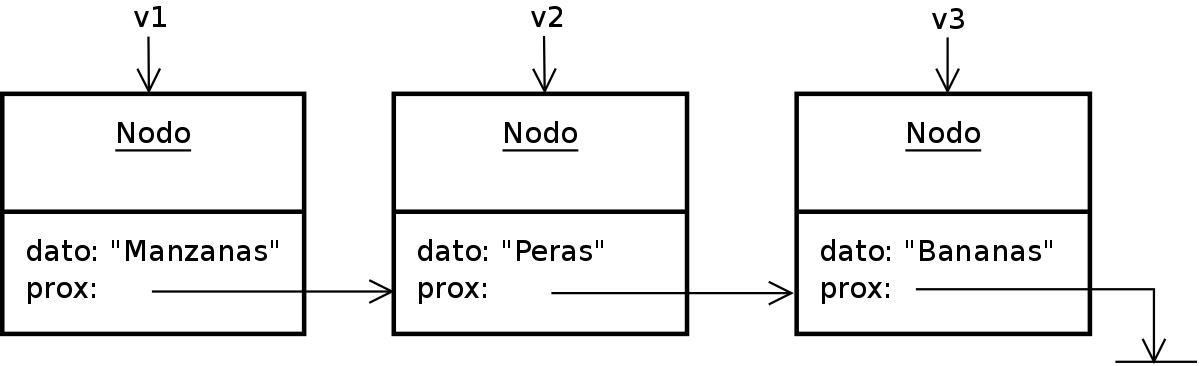
\includegraphics{graficos/16_Nodos}
\caption{Nodos enlazados}
\label{nodos}
\end{figure}

El atributo \lstinline!prox! de \lstinline!n3! tiene una referencia nula,
lo que indica que \lstinline!n3! es el último vagón de nuestra estructura.

Hemos creado una lista en forma manual. Si nos interesa recorrerla, podemos
hacer lo siguiente:

\begin{codigo-python-sn}
def ver_lista(nodo):
    """Recorre todos los nodos a través de sus enlaces,
       mostrando sus contenidos."""

    while nodo is not None:
        print(nodo)
        nodo = nodo.prox
\end{codigo-python-sn}

\begin{codigo-python-sn}
>>> ver_lista(n1)
Manzanas
Peras
Bananas
\end{codigo-python-sn}

Es interesante notar que la estructura del recorrido de la lista es el
siguiente:

\begin{itemize}
\item Se le pasa a la función sólo la referencia al primer nodo.

\item El resto del recorrido se consigue siguiendo la cadena de
referencias dentro de los nodos.
\end{itemize}

Si se desea {\it desenganchar} un vagón del medio de la lista, alcanza con
cambiar la referencia |prox|:

\begin{codigo-python-sn}
>>> n1.prox = n3
>>> ver_lista(n1)
Manzanas
Bananas
>>> n1.prox = None
>>> ver_lista(n1)
Manzanas
\end{codigo-python-sn}

De esta manera también se pueden generar estructuras impensables:
¿qué sucede si escribimos \lstinline!n1.prox = n1!? La representación es finita
y sin embargo en este caso \lstinline!ver_lista(n1)! no termina nunca. Hemos
creado una {\it lista infinita}, también llamada {\it lista circular}.

% Este ejercicio no se entiende
%\ejercicioc{¿Cuál es la mejor manera
%de tener siempre manzanas y peras a disposición de uno?}

\subsection{Caminos}

En una lista implementada con nodos, si seguimos las flechas
dadas por las referencias, obtenemos un {\it camino} en la lista.

Los caminos cerrados se denominan {\it ciclos}. Son ciclos, por ejemplo, la
autorreferencia de \lstinline|n1| a \lstinline|n1|, como así también una
flecha de \lstinline|n1| a \lstinline|n2| seguida de una flecha de
\lstinline|n2| a \lstinline|n1|.

\begin{atencion}
Las listas circulares no tienen nada de malo en sí mismas,
mientras su representación sea finita. El problema, en cambio, es que debemos tener
mucho cuidado al escribir programas para recorrerlas, ya que el recorrido
debe ser acotado (por ejemplo no habría problema en ejecutar un programa
que liste los 20 primeros nodos de una lista circular).

Cuando una función recibe una lista y el recorrido no está acotado,
se debe aclarar en su precondición que la ejecución de la misma terminará
sólo si la lista no contiene ciclos. Ése es el caso de la función
\lstinline|ver_lista(n1)|.
\end{atencion}

\subsection{Referenciando el principio de la lista}

Una cuestión no contemplada hasta el momento es la de mantener una referencia
a la lista completa. Por ahora para nosotros la lista es la colección de nodos
que se enlazan a partir de \lstinline|n1|. Sin embargo puede suceder que queramos
quitar a \lstinline|n1| y continuar con el resto de la lista como la colección de
nodos a tratar.

Una solución muy simple es asociar una referencia al principio de la lista,
que llamaremos \lstinline|lista|, y que mantendremos independientemente de cuál sea
el nodo que está al principio de la lista:

\begin{codigo-python-sn}
>>> n3 = Nodo("Bananas")
>>> n2 = Nodo("Peras", n3)
>>> n1 = Nodo("Manzanas", n2)
>>> lista = n1
>>> ver_lista(lista)
Manzanas
Peras
Bananas
\end{codigo-python-sn}

Ahora sí estamos en condiciones de eliminar el primer elemento de la lista
sin perder la identidad de la misma:

\begin{codigo-python-sn}
>>> lista = lista.prox
>>> ver_lista(lista)
Peras
Bananas
\end{codigo-python-sn}

\section{Tipos abstractos de datos}

Los tipos nuevos que habíamos definido en unidades anteriores fueron tipos de
datos concretos: un punto se definía como un par ordenado de números, un hotel
se definía por dos cadenas de caracteres (nombre y unicación) y dos números
(calidad y precio), etc.

Vamos a ver ahora una nueva manera de definir datos: por las
operaciones que tienen y por lo que tienen que hacer esas
operaciones (cuál es el resultado esperado de esas operaciones).

Esa manera de definir datos se conoce como {\it tipos abstractos de datos} o
{\it TADs}.

Lo novedoso de este enfoque respecto del anterior es que en general se puede
encontrar más de una representación mediante tipos concretos para representar
el mismo TAD, y que se puede elegir la representación más conveniente en cada
caso, según el contexto de uso.

Los programas que los usan hacen referencia a las operaciones que tienen, no a
la representación, y por lo tanto ese programa sigue funcionando si se cambia
la representación.

Dentro del ciclo de vida de un TAD hay dos fases: la programación del TAD y
la construcción de los programas que lo usan.

Durante la fase de programación del TAD, habrá que elegir una
representación, y luego programar cada uno de los métodos sobre esa
representación.

Durante la fase de construcción de los programas, no será relevante para el
programador que utiliza el TAD cómo está implementado, sino únicamente los
métodos que posee.

\begin{observacion}
Utilizando el concepto de \emph{interfaz} visto en la unidad anterior, podemos
decir que a quien utilice el TAD sólo le interesará la interfaz que éste
ofrezca.
\end{observacion}

\section{La clase {\tt ListaEnlazada}}

Basándonos en los nodos implementados anteriormente, pero buscando
desligar al programador que desea usar la lista de la responsabilidad de
manipular las referencias, definiremos ahora la clase
\lstinline!ListaEnlazada!, de modo tal que no haya que operar mediante las
referencias internas de los nodos, sino que se lo pueda hacer a través de
operaciones de lista.

Más allá de la implementación en particular, se podrá notar que implementaremos
los mismos métodos de las listas de Python, de modo que más allá del
funcionamiento interno, ambas serán {\bf listas}.

Definimos a continuación las operaciones que inicialmente deberá cumplir la
clase \lstinline!ListaEnlazada!.

\begin{itemize}
\item \lstinline|__str__|, para obtener una representación en cadena de texto.

\item \lstinline|__len__|, para calcular la longitud de la lista.

\item \lstinline|append(x)|, para agregar un elemento al final de la lista.

\item \lstinline|insert(i, x)|, para agregar el elemento \lstinline!x! en la
posición \lstinline!i! (levanta una excepción si la posición \lstinline!i! es
inválida).

\item \lstinline|remove(x)|, para eliminar la primera aparición de
\lstinline!x! en la lista (levanta una excepción si \lstinline!x! no está).

\item \lstinline|pop([i])|, para eliminar el elemento que está en la posición
\lstinline!i! y devolver su valor. Si no se especifica el valor de
\lstinline!i!, \lstinline|pop()| elimina y devuelve el elemento que está en
el último lugar de la lista (levanta una excepción si se hace referencia a
una posición no válida de la lista).

\item \lstinline|index(x)|, devuelve la posición de la primera aparición de
\lstinline!x! en la lista (levanta una excepción si \lstinline!x! no está).
\end{itemize}

Más adelante podrá agregarse a la lista otros métodos que también están
implementados por las listas de Python.

Valen ahora algunas consideraciones más antes de empezar a implementar la clase:

\begin{itemize}

\item Por lo dicho anteriormente, es claro que la lista deberá tener como
atributo la referencia al primer nodo que la compone.

\item Una implementación trivial del método |__len__| podría
recorrer todos los nodos de la lista y contar la cantidad de elementos,
pero si la lista tiene muchos elementos esto podría ser poco eficiente.

Para mejorar la eficiencia alcanza con agregar un atributo numérico que
contenga la cantidad de nodos. Así, este atributo que llamaremos |len|
se inicializará en $0$ cuando se cree la lista vacía, se
incrementará en $1$ cada vez que se agregue un elemento y se decrementará en $1$
cada vez que se elimine un elemento.

\begin{atencion}
Al agregar el atributo |len| estamos {\it duplicando información}, ya que habrá
dos formas de obtener la longitud de la lista:

\begin{enumerate}
\item contar los nodos
\item obtener el valor de |len|
\end{enumerate}

Como consecuencia, vamos a tener que prestar especial atención para que el
atributo |len| siempre contenga un valor consistente; es decir que su valor sea
siempre igual a la cantidad de nodos que contiene la lista.

En la sección \ref{invariante-objetos} se explica más formalmente este
concepto.
\end{atencion}

\item Por otro lado, como vamos a incluir todas las operaciones de listas
que sean necesarias para operar con ellas, no es necesario que la clase
\lstinline!Nodo! esté disponible para que otros programadores puedan
modificar (y romper) las listas a voluntad usando operaciones de nodos. Para eso
incluiremos la clase \lstinline!Nodo! de manera {\it privada} (es
decir oculta), de modo que la podamos usar nosotros como dueños
(fabricantes) de la clase, pero no cualquier programador que utilice la
lista.
\end{itemize}

Python tiene una convención para hacer que atributos, métodos o clases
dentro de una clase dada no puedan ser usados por los usuarios, y sólo
tengan acceso a ellos quienes programan la clase: su nombre tiene que
empezar con un guión bajo y terminar sin guión bajo. Así que para hacer que
los nodos sean privados, cambiaremos el nombre de la clase a \lstinline|_Nodo|.

\begin{observacion}
Se trata sólo de una convención, aun con el nombre \lstinline!_Nodo! la
clase está disponible, pero respetaremos esa convención de aquí en adelnte.
\end{observacion}

\subsection{Construcción de la lista}

Empezamos escribiendo la clase con su constructor.

\begin{codigo-python-sn}
class ListaEnlazada:
    """Modela una lista enlazada."""

    def __init__(self):
        """Crea una lista enlazada vacía."""
        # referencia al primer nodo (None si la lista está vacía)
        self.prim = None
        # cantidad de elementos de la lista
        self.len = 0
\end{codigo-python-sn}

Nuestra estructura ahora será como la representada por la Figura
\ref{lista_enlazada}.

\begin{figure}[htb]
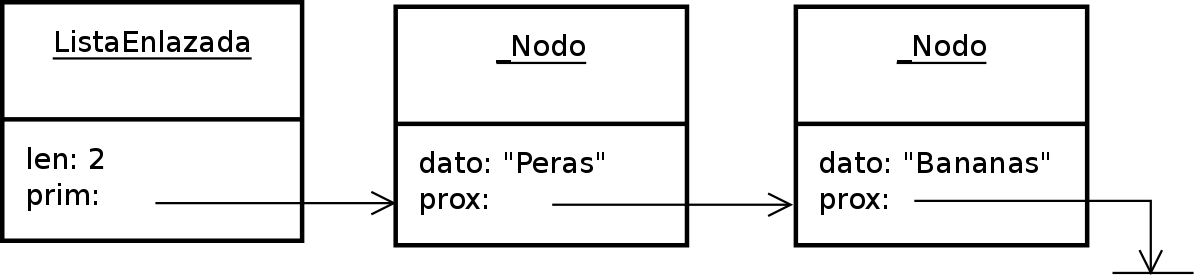
\includegraphics{graficos/16_ListaEnlazada}
\caption{Una lista enlazada}
\label{lista_enlazada}
\end{figure}

\ejercicioc{Escribir los métodos \lstinline!__str__! y \lstinline!__len__!
para la lista}.

\begin{sabias_que}
Una característica importante de la implementación de listas enlazadas es que
eliminar el primer elemento es una operación de {\it tiempo constante}, es
decir que no depende de la longitud de la lista. En las listas de
Python, por contraste, esta operación requiere un {\it tiempo proporcional a la
longitud de la lista}.

Sin embargo no todo es tan positivo: el acceso a la posición $p$ se realiza
en {\it tiempo proporcional a $p$}, mientras que en las listas de Python esta
operación se realiza en {\it tiempo constante}.

Conociendo las ventajas y desventajas podremos elegir el tipo de lista que
necesitemos según los requerimientos de cada problema.
\end{sabias_que}

\subsection{Eliminar un elemento de una posición}

Analizaremos a continuación \lstinline|pop([i])|, que elimina el elemento que
está en la posición \lstinline!i! y devuelve su valor. Si no se especifica
el valor de \lstinline!i!, \lstinline|pop()| elimina y devuelve el elemento
que está en el último lugar de la lista.  Por otro lado, levanta una
excepción si se hace referencia a una posición no válida de la lista.

Dado que se trata de una función con cierta complejidad, separaremos el
código en las diversas consideraciones a tener en cuenta.

\begin{itemize}

\item Si la posición es inválida (\lstinline!i! menor que $0$ o mayor o
igual a la longitud de la lista), se considera error y se levanta la
excepción |IndexError|.

Esto se resuelve con este fragmento de código:

\begin{codigo-python-sn}
if i < 0 or i >= self.len:
    raise IndexError("Índice fuera de rango")
\end{codigo-python-sn}

\item Si no se indica posición, \lstinline!i! toma la última posición de la
lista:

\begin{codigo-python-sn}
if i is None:
    i = self.len - 1
\end{codigo-python-sn}

\item Cuando la posición es $0$ se trata de un caso particular, ya que en ese
caso hay que cambiar la referencia de
\lstinline!self.prim! para que apunte al nodo siguiente.  Es decir, pasar de
\lstinline!self.prim! $\rightarrow$ |nodo0| $\rightarrow$ |nodo1| a
\lstinline!self.prim! $\rightarrow$ |nodo1|).

\begin{codigo-python-sn}
if i == 0:
    dato = self.prim.dato
    self.prim = self.prim.prox
\end{codigo-python-sn}

\noindent (Guardamos el |dato| del nodo descartado para poder devolverlo al
finalizar la función).

\item Vemos ahora el caso general:

Mediante un ciclo, se deben ubicar los nodos $n_{i - 1}$ y $n_i$ que
están en las posiciones $i-1$ e $i$ de la lista, respectivamente, de modo de
poder ubicar no sólo el nodo que se descartará, sino también estar en condiciones
de saltear el nodo descartado en los enlaces de la lista.  La lista debe pasar de
contener el camino $n_{i-1} \rightarrow n_i \rightarrow n_{i+1}$
a contener el camino $n_{i-1} \rightarrow n_{i+1}$.

Nos basaremos un esquema muy simple y útil que se denomina {\it máquina de parejas}:

Si nuestra secuencia tiene la forma $ABCDE$, se itera sobre ella de modo de
tener las parejas $AB$, $BC$, $CD$, $DE$. En la pareja $XY$, llamaremos a $X$ el
{\it elemento anterior}
y a $Y$ el {\it elemento actual}. En general estos ciclos terminan o bien cuando
no hay más parejas que formar, o bien cuando el elemento actual cumple con una determinada
condición.

En nuestro problema, tenemos la siguiente situación:

\begin{itemize}
\item Las parejas son parejas de nodos.

\item Para avanzar en la secuencia se usa la referencia al próximo nodo de la lista.

\item La condición de terminación es siempre que la posición del nodo en la
lista sea igual al valor buscado.  En este caso particular no debemos
preocuparnos por la terminación de la lista porque la validez del índice
buscado ya fue verificada más arriba.
\end{itemize}

Esta es la porción de código correspondiente a la búsqueda. Llamamos |n_ant| y
|n_act| a los elementos anterior y actual de la pareja de nodos:

\begin{codigo-python-sn}
n_ant = self.prim
n_act = n_ant.prox
for pos in xrange(1, i):
    n_ant = n_act
    n_act = n_ant.prox
\end{codigo-python-sn}

Al finalizar el ciclo, \lstinline!n_ant! será una referencia al nodo $i-1$ y
\lstinline!n_act! una referencia al nodo $i$.

Una vez obtenidas las referencias, se obtiene el dato y se cambia el camino
para descartar el nodo |n_act|:

\begin{codigo-python-sn}
dato = n_act.dato
n_ant.prox = n_act.prox
\end{codigo-python-sn}

\item Finalmente, en todos los casos de éxito se debe devolver el dato que contenía
el nodo descartado y decrementar la longitud en 1:

\begin{codigo-python-sn}
self.len -= 1
return dato
\end{codigo-python-sn}

\end{itemize}

Finalmente, en el Código \ref{lista_enlazada_pop} se incluye el código completo
del método \lstinline!pop!.

\begin{codigo}{pop}{Método pop de la lista enlazada}
\label{lista_enlazada_pop}
\begin{codigo-python}
def pop(self, i=None):
    """Elimina el nodo de la posición i, y devuelve el dato contenido.
       Si i está fuera de rango, se levanta la excepción IndexError.
       Si no se recibe la posición, devuelve el último elemento."""

    if i is None:
        i = self.len - 1

    if i < 0 or i >= self.len:
        raise IndexError("Índice fuera de rango")

    if i == 0:
        # Caso particular: saltear la cabecera de la lista
        dato = self.prim.dato
        self.prim = self.prim.prox
    else:
        # Buscar los nodos en las posiciones (i-1) e (i)
        n_ant = self.prim
        n_act = n_ant.prox
        for pos in xrange(1, i):
            n_ant = n_act
            n_act = n_ant.prox

        # Guardar el dato y descartar el nodo
        dato = n_act.dato
        n_ant.prox = n_act.prox

    self.len -= 1
    return dato
\end{codigo-python}
\end{codigo}

\subsection{Eliminar un elemento por su valor}

Análogamente se resuelve \lstinline|remove(self, x)|, que debe eliminar la
primera aparición de \lstinline!x! en la lista, o bien levantar una excepción
si \lstinline!x! no se encuentra en la lista.

Nuevamente, dado que se trata de un método de cierta complejidad, lo
resolveremos por partes, teniendo en cuenta los casos particulares y el caso
general.

\begin{itemize}

\item Si la lista está vacía levantamos una excepción. Tenemos que tratarlo
como un caso particular, ya que en todos los siguientes casos necesitamos
que haya al menos un nodo.

\begin{codigo-python-sn}
if self.prim is None
    raise ValueError("La lista está vacía")
\end{codigo-python-sn}

\item El caso en el que x está en el primer nodo también es particular, ya
que modificar la referencia |self.prim|:

\begin{codigo-python-sn}
if self.prim.dato == x:
    self.prim = self.prim.prox
\end{codigo-python-sn}

\item El caso general también implica un recorrido con máquina de parejas, sólo
que esta vez la condición de terminación es: o bien la lista se terminó o bien
encontramos un nodo con el valor \lstinline!x! buscado.

\begin{codigo-python-sn}
n_ant = self.prim
n_act = n_ant.prox
while n_act is not None and n_act.dato != x:
    n_ant = n_act
    n_act = n_ant.prox
\end{codigo-python-sn}

En este caso, al terminarse el ciclo será necesario corroborar si se terminó
porque llegó al final de la lista, y de ser así levantar una excepción; o si se
terminó porque encontró el dato, y de ser así eliminarlo.

\begin{codigo-python-sn}
if n_act is None:
    raise ValueError("El valor no está en la lista.")
n_ant.prox = n_act.prox
\end{codigo-python-sn}

\item Finalmente, en todos los casos de éxito debemos decrementar en 1 el valor
de \lstinline|self.len|.

\end{itemize}

En el Código \ref{lista_enlazada_remove} se incluye el código completo
del método \lstinline!remove!.

\begin{codigo}{remove}{Método remove de la lista enlazada}
\label{lista_enlazada_remove}
\begin{codigo-python}
def remove(self, x):
    """Borra la primera aparición del valor x en la lista.
       Si x no está en la lista, levanta ValueError"""

    if self.len == 0:
        raise ValueError("Lista vacía")

    if self.prim.dato == x:
        # Caso particular: saltear la cabecera de la lista
        self.prim = self.prim.prox
    else:
        # Buscar el nodo anterior al que contiene a x (n_ant)
        n_ant = self.prim
        n_act = n_ant.prox
        while n_act is not None and n_act.dato != x:
            n_ant = n_act
            n_act = n_ant.prox

        if n_act == None:
            raise ValueError("El valor no está en la lista.")

        # Descartar el nodo
        n_ant.prox = n_act.prox

    self.len -= 1
\end{codigo-python}
\end{codigo}

\subsection{Insertar nodos}

Debemos programar ahora \lstinline|insert(i, x)|, que debe agregar el elemento
\lstinline!x! en la posición \lstinline!i!  (y levantar una excepción si la
posición \lstinline!i! es inválida).

Veamos qué debemos tener en cuenta para programar esta función.

\begin{itemize}

\item Si se intenta insertar en una posición menor que cero o mayor que la
longitud de la lista debe levantarse una excepción.

\begin{codigo-python-sn}
if i < 0 or i > self.len:
    raise IndexError("Posición inválida")
\end{codigo-python-sn}

\item Para los demás casos hay que crear un nodo, que será el que se insertará
en la posición que corresponda. Construimos un nodo \lstinline|nuevo| cuyo
\lstinline|dato| será \lstinline|x|.

\begin{codigo-python-sn}
nuevo = _Nodo(x)
\end{codigo-python-sn}

\item Si se quiere insertar en la posición 0, hay que cambiar la referencia de
\lstinline|self.prim|.

\begin{codigo-python-sn}
if i == 0:
    nuevo.prox = self.prim
    self.prim = nuevo
\end{codigo-python-sn}

\item Para los demás casos, nuevamente será necesaria la máquina de parejas.
Obtenemos el nodo anterior a la posición en la que queremos insertar.

\begin{codigo-python-sn}
n_ant = self.prim
for pos in xrange(1, i):
    n_ant = n_ant.prox

nuevo.prox = n_ant.prox
n_ant.prox = nuevo
\end{codigo-python-sn}

\item En todos los casos de éxito se debe incrementar en 1 la longitud de la lista.

\end{itemize}

En el Código \ref{lista_enlazada_insert} se incluye el código resultante
del método \lstinline!insert!.

\begin{codigo}{insert}{Método insert de la lista enlazada}
\label{lista_enlazada_insert}
\begin{codigo-python}
def insert(self, i, x):
    """Inserta el elemento x en la posición i.
       Si la posición es inválida, levanta IndexError"""

    if i < 0 or i > self.len:
        raise IndexError("Posición inválida")

    nuevo = _Nodo(x)

    if i == 0:
        # Caso particular: insertar al principio
        nuevo.prox = self.prim
        self.prim = nuevo
    else:
        # Buscar el nodo anterior a la posición deseada
        n_ant = self.prim
        for pos in xrange(1, i):
            n_ant = n_ant.prox

        # Intercalar el nuevo nodo
        nuevo.prox = n_ant.prox
        n_ant.prox = nuevo

    self.len += 1
\end{codigo-python}
\end{codigo}

\ejercicioc{Completar la clase \lstinline|ListaEnlazada| con los métodos que
faltan: \lstinline|append| e \lstinline|index|}.

\ejercicioc{En los bucles de {\it máquina de parejas} mostrados
anteriormente, no siempre es necesario tener la referencia al nodo actual,
puede alcanzar con la referencia al nodo anterior.  Donde sea posible,
eliminar la referencia al nodo actual.  Una vez hecho esto, analizar el
código resultante, ¿Es más elegante?}

\ejercicioc{\label{append_constante} {\bf Mantenimiento:} Con esta representación conseguimos que la
inserción en la posición 0 se realice en tiempo constante, sin embargo ahora
\lstinline|append| es lineal en la longitud de la lista. Si queremos mejorar
esto, debemos agregar un atributo más a los objetos de la
clase: la referencia al último nodo, y modificar \lstinline|append| para que se
pueda ejecutar en tiempo constante. Por supuesto que además hay que modificar
todos los métodos de la clase para que se mantenga la propiedad de que ese
atributo siempre es una referencia al útimo nodo.}

\section{Invariantes de objetos}

\label{invariante-objetos}
Los invariantes son condiciones que deben ser siempre ciertas.  En la sección
\label{invariantes} mencionamos los invariantes de ciclos, que son condiciones que deben
permanecer ciertas durante la ejecución de un ciclo.  Existen también los
invariantes de objetos, que son condiciones que deben ser ciertas a lo
largo de toda la existencia de un objeto.

La clase \lstinline!ListaEnlazada! presentada en la sección anterior,
cuenta con dos invariantes que siempre debemos mantener.  Por un lado, el
atributo \lstinline!len! debe contener siempre la cantidad de nodos de la
lista.  Es decir, siempre que se modifique la lista, agregando o quitando
un nodo, se debe actualizar \lstinline!len! como corresponda.

Por otro lado, el atributo \lstinline!prim! referencia siempre al primer
nodo de la lista. Si se agrega o elimina este primer nodo, es necesario
actualizar esta referencia.

Cuando se desarrolla una estructura de datos como la lista enlazada, es
importante destacar cuáles serán sus invariantes, ya que en cada método
habrá que tener especial cuidado de que los invariantes permanezcan siempre
ciertos.

Así, si se modifica la lista para que la inserción al final pueda hacerse en
tiempo constante (como se pide en el ejercicio \ref{append_constante}),
se está agregando a la lista un nuevo invariante (un atributo de la lista
que apunte siempre al último elemento) y no es sólo el método
\lstinline!append! el que hay que modificar, sino todos los métodos que
puedan de una u otra forma cambiar la referencia al último elemento de la
lista.

\section{Otras listas enlazadas}

Las listas presentadas hasta aquí son las {\it listas simplemente
enlazadas}, que son sencillas y útiles cuando se quiere poder insertar o
eliminar nodos de una lista en tiempo constante.

Existen otros tipos de listas enlazadas, cada uno con sus ventajas y
desventajas.

\subsection*{Listas doblemente enlazadas}

Las listas doblemente enlazadas son aquellas en que los nodos cuentan no
sólo con una referencia al siguiente, sino también con una referencia al
anterior.  Esto permite que la lista pueda ser recorrida en ambas
direcciones.

En una lista doblemente enlazada es posible, por ejemplo, eliminar un
nodo sin necesidad de saber cuál es el anterior.

Entre las desventajas podemos mencionar que al tener que mantener dos
referencias el código se vuelve más complejo, y también que ocupa más
espacio en memoria.

\subsection*{Listas circulares}

Las listas circulares, que ya fueron mencionadas al comienzo de esta
unidad, son aquellas en las que el último nodo contiene una referencia al
primero.  Pueden ser tanto simplemente como doblemente enlazadas.

Se las utiliza para modelar situaciones en las cuales los elementos no
tienen un primero o un último, sino que forman una cadena infinita, que se
recorre una y otra vez.

\begin{sabias_que}
El código del kernel Linux, que está programado en C, incluye una
implementación de lista enlazada circular utilizada en la mayoría de los
subsistemas.

Por ejemplo, la lista de tareas que se están ejecutando es una lista
circular.  El {\it scheduler} (planificador) del kernel permite que cada tarea
utilice el procesador durante una porción de tiempo y luego pasa a la
siguiente, aplicando así una ``ronda de turnos'' sin que haya una primera o una
última tarea.
\end{sabias_que}

\section{Iteradores}

En la unidad anterior se hizo referencia a que todas las secuencias
pueden ser recorridas mediante una misma estructura
(\lstinline!for variable in secuencia!), ya que todas implementan el método
especial \lstinline!__iter__!.  Este método debe devolver un {\it iterador}
capaz de recorrer la secuencia como corresponda.

\begin{observacion}
Un iterador es un objeto que permite recorrer uno a uno los elementos
almacenados en una estructura de datos, y operar con ellos.
\end{observacion}

Un ejemplo de iteradores que estuvimos usando desde la primera unidad es la
función |range|:

\begin{codigo-python-sn}
>>> r = range(3)
>>> type(r)
<class 'range'>
\end{codigo-python-sn}

Lo primero que observamos es que la función |range| no devuelve una lista de
números, sino que devuelve una instancia de la clase |range|. Para obtener un
iterador a partir de este objeto podemos aplicar la función |iter| (que a su
vez llamará al método |__iter__|):

\begin{codigo-python-sn}
>>> i = iter(r)
>>> type(i)
<class 'range_iterator'>
\end{codigo-python-sn}

En Python los iteradores implementan un método
\lstinline!__next__! que debe devolver los elementos, de a uno por vez,
comenzando por el primero.  Y al llegar al final de la estructura, debe
levantar una excepción de tipo \lstinline!StopIteration!.

La función |next| permite invocar manualmente al método |__next__|:

\begin{codigo-python-sn}
>>> next(i)
0
>>> next(i)
1
>>> next(i)
2
>>> next(i)
Traceback (most recent call last):
  File "<stdin>", line 1, in <module>
StopIteration
\end{codigo-python-sn}

Cuando hacemos |for x in range(3)|, el bucle |for| automáticamente llama a las
funciones |iter| y |next|, asignando a |x| los valores que devuelve |next| en
cada iteración.

Es decir que las siguientes estructuras son equivalentes:

\begin{codigo-python-sn}
for elemento in secuencia:
	# hacer algo con elemento
\end{codigo-python-sn}

\begin{codigo-python-sn}
iterador = iter(secuencia)
while True:
    try:
        elemento = next(iterador)
    except StopIteration:
        break
    # hacer algo con elemento
\end{codigo-python-sn}

\subsection*{Iterador para la lista enlazada}

Si queremos implementar un iterador para la lista enlazada,
la mejor solución implica crear una nueva clase,
\lstinline!_IteradorListaEnlazada!, que implemente el método
\lstinline!__next__! de la forma apropiada.

\begin{atencion}
Utilizamos la notación de clase privada, utilizada también para la clase
\lstinline!_Nodo!, ya que si bien se devolverá el iterador cuando sea
necesario, un programador externo no debería construir el iterador sin
pasar a través de la lista enlazada.
\end{atencion}

Para inicializar la clase, lo único que se necesita es una referencia al
primer elemento de la lista.

\begin{codigo-python-sn}
class _IteradorListaEnlazada:
    def __init__(self, prim):
        self.actual = prim
\end{codigo-python-sn}

A partir de allí, el iterador irá avanzando a través de los elementos de la
lista mediante el método \lstinline!__next__!.  Para verificar que no se haya
llegado al final de la lista, se corroborará que la referencia
\lstinline!self.actual! sea distinta de \lstinline!None!.

\begin{codigo-python-sn}
if self.actual is None:
    raise StopIteration()
\end{codigo-python-sn}

Una vez que se pasó la verificación, la primera llamada a \lstinline!__next__!
debe devolver el primer elemento, pero también debe avanzar, para que la
siguiente llamada devuelva el siguiente elemento.  Por ello, se utiliza la
estructura {\it guardar, avanzar, devolver}.

\begin{codigo-python-sn}
dato = self.actual.dato
self.actual = self.actual.prox
return dato
\end{codigo-python-sn}

En el Código \ref{iterador_enlazada} se puede ver el código completo del
iterador.

\begin{codigo}{\_IteradorListaEnlazada}{Un iterador para la lista enlazada}
\label{iterador_enlazada}
\begin{codigo-python}
class _IteradorListaEnlazada:
    def __init__(self, prim):
        self.actual = prim

    def __next__(self):
        if self.actual is None:
            raise StopIteration()

        dato = self.actual.dato
        self.actual = self.actual.prox
        return dato
\end{codigo-python}
\end{codigo}

Finalmente, es necesario modificar la clase \lstinline!ListaEnlazada! para que
devuelva una instancia del iterador
cuando se llama al método \lstinline!__iter__!.

\begin{codigo-python-sn}
    def __iter__(self):
        """Devuelve un iterador de la lista."""
        return _IteradorListaEnlazada(self.prim)
\end{codigo-python-sn}

Con todo esto será posible recorrer nuestra lista con la estructura a la
que estamos acostumbrados.

\begin{codigo-python-sn}
>>> l = ListaEnlazada()
>>> l.append(7)
>>> l.append(3)
>>> l.append(5)
>>> for valor in l:
...     print(valor)
...
7
3
5
\end{codigo-python-sn}

No solo eso, sino que además podremos utilizar la lista enlazada en cualquier
operación que requiera una secuencia {\it iterable}:

\begin{codigo-python-sn}
>>> list(l) # convertir a una lista de Python
[7, 3, 5]
>>> sum(l) # sumar los elementos
15
>>> max(l) # obtener el máximo elemento
7
\end{codigo-python-sn}

\section{Resumen}

\begin{itemize}

\item Un {\bf tipo abstracto de datos} (TAD) es un tipo de datos que está
definido por las operaciones que contiene y cómo se comportan (su {\it
interfaz}), no por la forma en la que esas operaciones están implementadas.

\item Una {\bf lista enlazada} es una implementación del TAD {\it lista}.
Se trata de una lista compuesta por nodos, en la que
cada nodo contiene un dato y una referencia al nodo que le sigue.

\item En las listas enlazadas, es {\it barato} insertar o eliminar
elementos, ya que simplemente se deben alterar un par de referencias; pero
es {\it caro} acceder a un elemento en particular, ya que es necesario
pasar por todos los anteriores para llegar a él.

\item Tanto al insertar como al remover elementos de una lista enlazada, se
utiliza la técnica de {\it máquina de parejas}, mediante la cual se va
recorriendo la lista hasta encontrar el lugar apropiado donde operar con
las referencias.

\item Una {\bf lista doblemente enlazada} es aquella cuyos nodos además del
dato contienen una referencia al nodo anterior y otra al nodo siguiente, de
modo que se la puede recorrer en ambos sentidos.

\item Una {\bf lista circular} es aquella en la que el último nodo contiene
una referencia al primero, y puede ser recorrida infinitamente.

\item Un {\bf iterador} es un objeto que permite recorrer uno a uno los
elementos de una secuencia.

\end{itemize}

\begin{referencia_python}

\begin{sintaxis}{\lstinline{__iter__(self)}}
Método especial que debe devolver un iterador para el objeto. El iterador debe
ser un objeto que implementa el método |__next__|.
\end{sintaxis}

\begin{sintaxis}{\lstinline{__next__(self)}}
Devuelve el elemento actual de la iteración y avanza al siguiente.
Si se llegó al final de la iteración lanza |StopIteration|.
\end{sintaxis}

\begin{sintaxis}{\lstinline{iter(objeto)}}
Equivalente a invocar |objeto.__iter__()|.
\end{sintaxis}

\begin{sintaxis}{\lstinline{next(objeto, [valor])}}
Equivalente a invocar |objeto.__next__()|. Si se invoca con el parámetro
adicional |valor|, al llegar al final de la iteración se devuelve el |valor| en
lugar de lanzar |StopIteration|.
\end{sintaxis}
\end{referencia_python}

\newpage
\section{Ejercicios}

\extractionlabel{guia}
\begin{ejercicio}
Agregar a la clase {\it ListaEnlazada} un método \verb!next! que vaya
devolviendo uno a uno cada elemento de la lista, desde el primero hasta el
último.  Al llegar al final de la lista debe levantar una excepción de la
clase {\it StopIteration}.  Para el correcto funcionamiento de este método, ¿es
necesario agregar un atributo adicional a la clase?
\end{ejercicio}

\extractionlabel{guia}
\begin{ejercicio}
Utilizando el método \verb!next! del ejercicio anterior, redefinir el
método \verb!__str__! de {\it ListaEnlazada}, para que se genere una salida
legible de lo que contiene la lista, similar a las listas de python. \\
{\bf Nota}: este método debe devolver una cadena, no imprimirla por
pantalla.
\end{ejercicio}

\extractionlabel{guia}
\begin{ejercicio}
Agregar a {\it ListaEnlazada} un método \verb!extend! que reciba una {\it
ListaEnlazada} y agregue a la lista actual los elementos que se encuentran
en la lista recibida.
\end{ejercicio}

% No es un buen ejemplo que LE Ordenada herede de LE ya que se tiene que bloquear
% o redefinir el significado del método append.
%
%\ejercicioc{
%Escribir una clase {\it ListaEnlazadaOrdenada} que herede de {\it
%ListaEnlazada}, redefiniendo el método \verb!insert! para que inserte los
%elementos de forma ordenada, y el método \verb!append! para que no permita
%la inserción al final.
%}

\extractionlabel{guia}
\begin{ejercicio}
Una {\bf lista circular} es una lista cuyo último nodo está ligado al primero,
de modo que es posible recorrerla infinitamente.  \\
Escribir la clase {\it ListaCircular}, incluyendo los métodos \verb!insert!,
\verb!append!, \verb!remove! y \verb!pop!.
\end{ejercicio}

\extractionlabel{guia}
\begin{ejercicio}
Una {\bf lista doblemente enlazada} es una lista en la cual cada nodo tiene
una referencia al anterior además de al próximo de modo que es posible
recorrerla en ambas direcciones. \\
Escribir la clase {\it ListaDobleEnlazada}, incluyendo los métodos
\verb!insert!, \verb!append!, \verb!remove! y \verb!pop!.
\end{ejercicio}

\extractionlabel{guia}
\begin{ejercicio}
Escribir un método de la clase {\it ListaEnlazada} que invierta el orden
de la lista (es decir, el primer elemento queda como último y
viceversa, y se invierte la dirección de todos los enlaces). \\
{\bf Nota}: operar directamente sobre los elementos de la lista.
\end{ejercicio}

